\pdfsuppresswarningpagegroup=1

\documentclass[11pt]{article}

\usepackage{cite}
\usepackage{graphicx}
\usepackage{float}
\usepackage{pdfpages}
\usepackage{bookmark}
\usepackage[top=1in,bottom=1in,left=1in,right=1in]{geometry} 

\hypersetup{
	colorlinks = true,
	linkcolor = blue,
	filecolor = magenta,
	urlcolor = cyan,
	citecolor = blue,
	pdftitle = {Gambling Report},
	pdfpagemode = UseOutlines,
}

\begin{document}
	\title{ \vspace{-1in}The Leftovers \\
			\Large{Part 3} }

	\author{	Nicholas Chiapputo, Khaemon Edwards, Caleb Halter, \\
				Jacob Robbins, Ryan Vanek, Saidat Babatunde, \\
				Ephraim Emilimor, Jordan Simmons
	}

	\maketitle

	\section{Introduction}
		Our restaurant management system is hosted through a live server at \cite{website}. The home page of the website has collapsible sections that we originally used to test the backend functionality while the frontend was being developed. We have left it there to more easily showcase each of the functionalities of the system. Some things, such as messaging and editing items, are not as easy to show, however. To get to any of the four user screens, simply use the menu bar. The kitchen option will take you directly to the single kitchen page where orders are queried every 5 seconds. The manager option will take you to a login screen for managers and similarly for the server option. If you would like to test logging in, please use the employees tab on the homepage to query the employee list. Retrieve the employee list under the ``Get Employees'' subheading. The login for an employee uses the ``\_id'' value as the username and the four-digit pin as a password. 

		When selecting the customer option, you will be taken to a login screen for the table. The idea behind this is that the restaurant management or staff will set up the systems in the morning (akin to turning the registers on). They will then set the system to the appropriate table. After the table is logged in (using ID values from 1 to 20, inclusively), the customer is unable to go back to the table login page. This prevents a customer from ordering for another table.

		The source files for our project can be found at \cite{repository} under the \texttt{src/} subdirectory. This is a combination of the client and backend sources. Some packages (e.g., formidable) may be necessary to install using \texttt{npm} to run correctly. Additionally, our site is using MongoDB to control database operations and NodeJS to interface between client requests and the backend operations. 

		Our unit tests were performed using JEST, a JavaScript testing framework. This was done through \texttt{npm} using some non-default packages including \texttt{frisby}. These can all be tested repeatedly to ensure functionality. There may be some difficulties with creating and editing menu items as these require file uploads. The test scripts themselves have a reference to one of the images included in our source files. So, if the hierarchy is maintained, all 80 unit tests will likely pass barring any unforeseen local issues.

	\section{Validation Tests}
		Attached following this description is a table of all validation tests we carried out.To the best of our ability, we tested that each and every one of these tests passed with expected results. Admittedly, there may be some unknown issues regarding non-ideal inputs that we have yet to find and fix. However, when considering ideal inputs, we believe that all 49 of these validation tests pass correctly. Below is a list of each validation test, the corresponding requirement from our requirements document, a description of the testing steps, the expected output, the comments regarding the testing, and whether or not it passed or failed at the time of submission.
	
		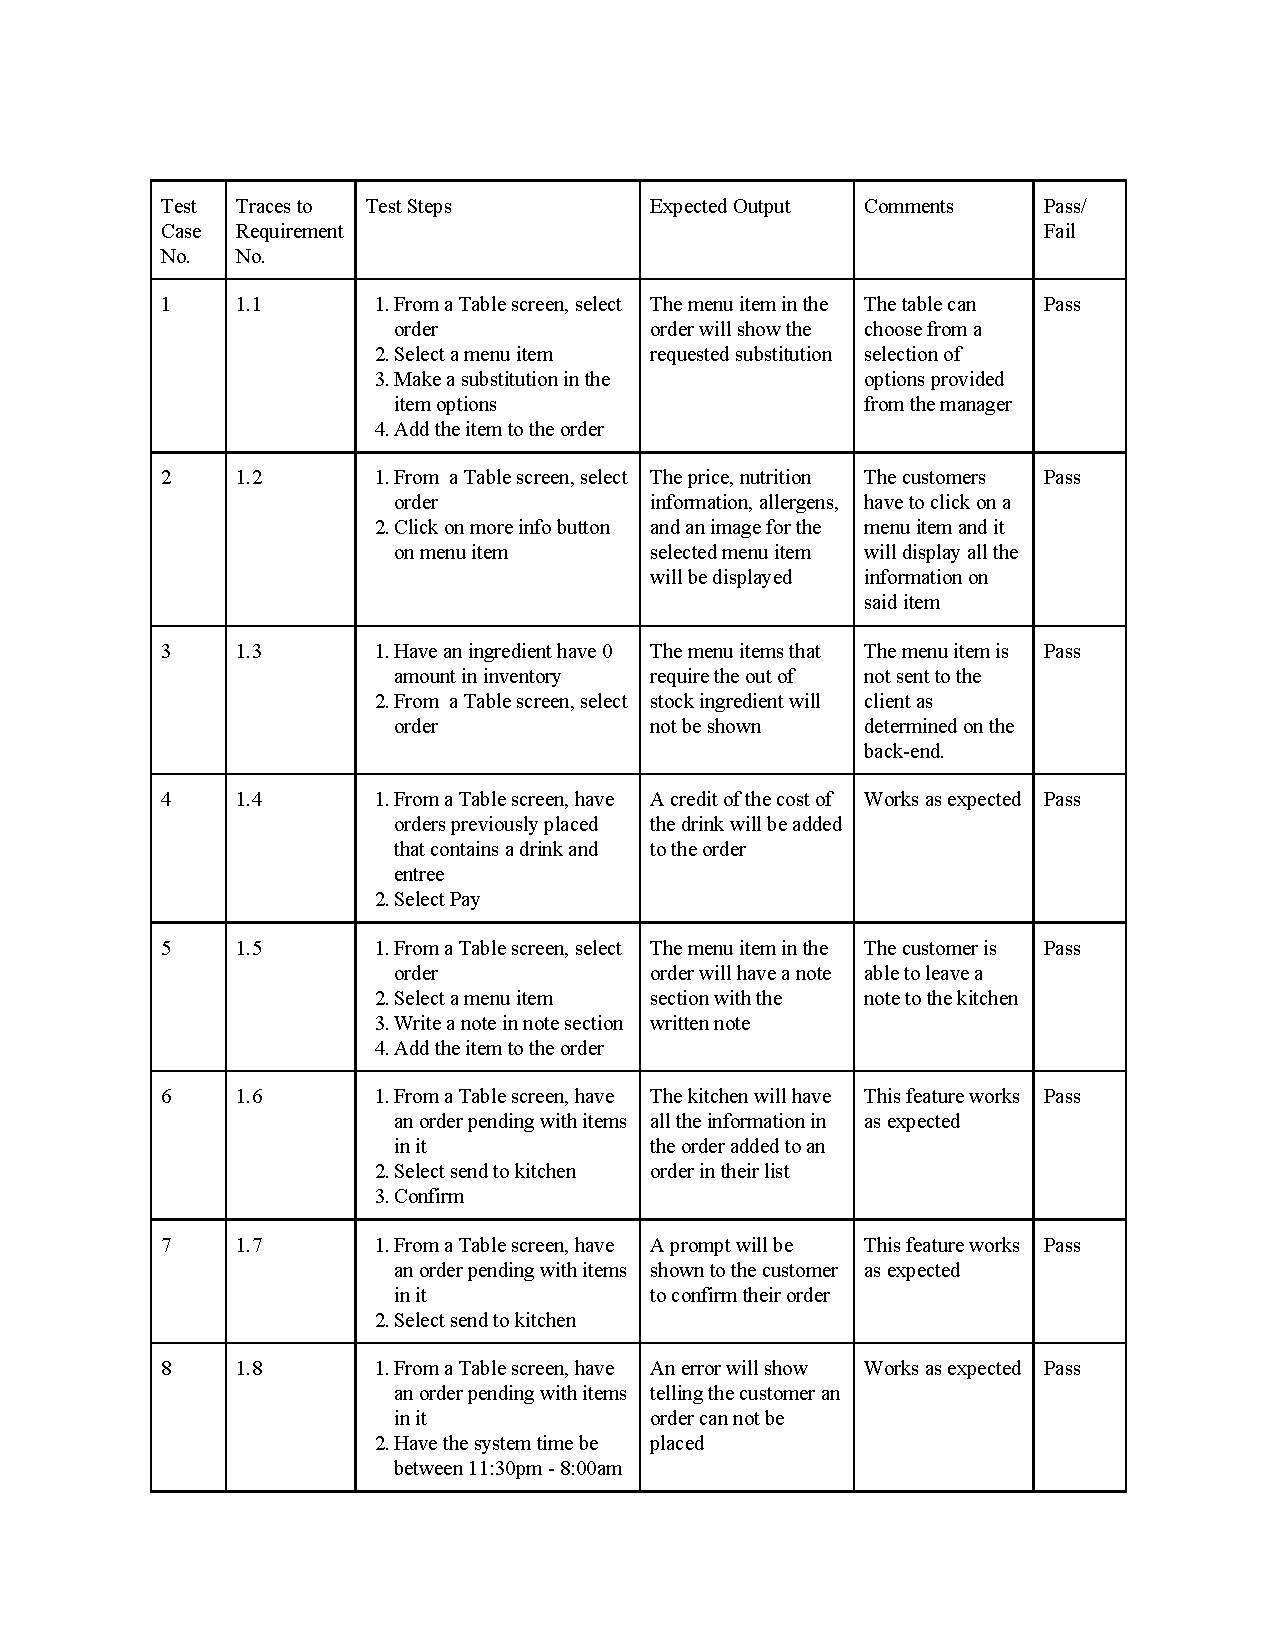
\includepdf[pages=-,pagecommand=\thispagestyle{plain}]{ValidationTests}

	\section{Unit Tests}
		The unit tests were performed using the JavaScript testing framework JEST. This was done through \texttt{npm} using some non-default packages including \texttt{frisby}. These can all be tested repeatedly to ensure functionality. There may be some difficulties with creating and editing menu items as these require file uploads. The test scripts themselves have a reference to one of the images included in our source files. So, if the hierarchy is maintained, all 80 unit tests will likely pass barring any unforeseen local issues. All of the scripts used for testing are located in the \texttt{src/UnitTests/} directory from \cite{repository}.

		The results of the tests are included with this document in the file `results.txt'. This file contains a prettified JSON-formatted result directly from JEST. The attributes The first 10 attributes represents the result of all test cases and test suites (each test suite is a file, and there are test cases within each file). The results of this show that we performed 80 tests in 11 test suites. All of these passed. 

		The test results for each unit test begins in the array on line 31 with the attribute ``testResults''. Each JSON object in this array is a single test suite. To explain the structure, we will consider the first object from line 32 to line 88. The ``assertionResults'' object is an array of JSON objects where each object represents a single test. Each of these objects has a ``fullName'' attribute that is a description of what the test is performing. For example, the first object in the first test suite, beginning on line 34 and going through line 41, is has the description ``Get teh list of orders from the order database.'' This test queries the server's order database and tests for a proper response. 

		Each object also has a ``status'' attribute whose value representes the result of the test. Since all of our tests passed, this attribute has the value ``passed'' for each of the 80 test cases. At the end of each test suite JSON block (e.g., lines 83-89 for the first suite), there is another ``status'' attribute. Since all of our test suites passed, this will have the value ``passed'' for each of the 11 test suites. This pattern continues for the rest of the results document, showing the passing status of each of the test cases and test suites.

	\begin{thebibliography}{00}
		\bibitem{website} [Online].Available: \url{http://64.225.29.130}
		\bibitem{repository} [Online].Available: \url{https://github.com/NickChiapputo/TheLeftovers/tree/master/src}
	\end{thebibliography}
\end{document}